\section{Tehnologije}
Za implementaciju rada izabran je Python programski jezik, koji je u posljednih godina dosegnuo visoku popularnost i koristi se u gotovo svim vrstama aplikacija. Interpretirani je jezik visoke razine opće namjene te ima filozofiju dizajna koji naglašava čitljivost k\^oda. Podržava više paradigme programiranja, uključujući objektno orijentirane, imperativne, funkcionalne i proceduralne. Programski jezik se dinamičko kuca (eng. \textit{dynamically typed}), što znači da se varijablama ne određuje tip, ali ako se želi postoji mogućnost izričito ga naglasiti. Posjeduje sveobuhvatnu biblioteku, koja između ostalog pokriva i područje umjetne inteligencije. Korištenjem se dosta olakšavaju obrade i pripreme podataka za inteligentne agente, te izradu istih. Također, kako se nebi sukobili paketi iz ovog projekta sa paketima iz drugog ili iz sustava, stvorilo se posebno virtualno okruženje samo za ovaj projekt. Pythonov modul koji to omogućuje zove se \emph{virtualenv}.

\subsection{Integrirano razvojno okruženje}
K\^od je pisan u razvojnom okruženju PyCharm koji je jedan od mnogih okruženja Češke tvrtke JetBrains. Glavne značajke su analiza k\^oda, grafički program za otklanjanje pogrešaka, integrirani tester jedininca te integracija s kontrolnim sustavom za verzioniranje. Izgled PyCharm integriranog razvojnog okruženja prikazan je na slici~\ref{fig:pycharm}.
\\[\intextsep]
\begin{minipage}{\linewidth}
	\centering%
	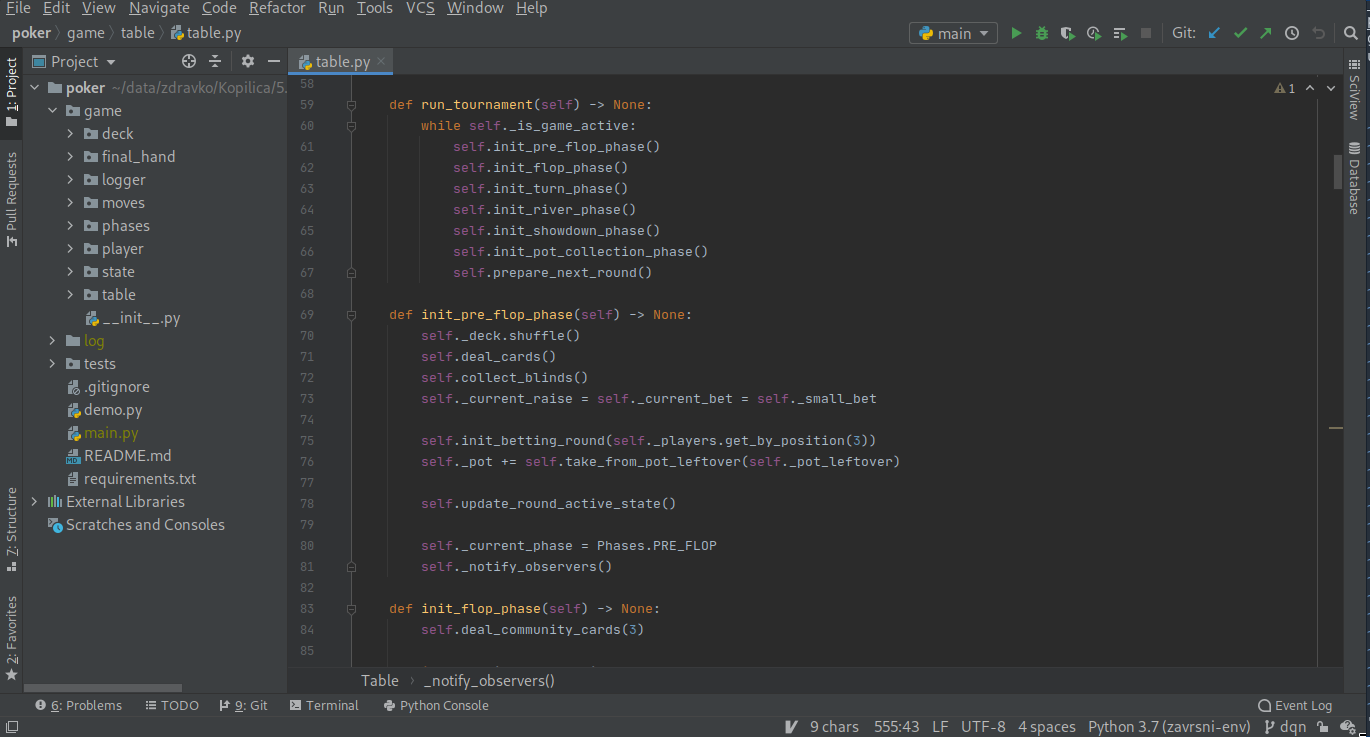
\includegraphics[width=0.8\linewidth,clip=]{images/pycharm.png}%
	\figcaption{Integrirano razvojno okruženje PyCharm}%
	\label{fig:pycharm}%
\end{minipage}
\\[\intextsep]

\subsection{Sustav za upravljanje verzijama}
Za praćenje promjena u izvornom k\^odu, korišten je git. Slobodan je i otvorenog k\^oda. Prilagođen je za rad programera, bilo to rade li više ljudi na istom projektu ili samo jedan, s tim da nije nužno da ga se koristi samo za praćenje promjene u izvornom k\^odu, nego za bilo koju vrstu datoteka. Osnovne značajke su mu brzina, integracija podataka, te podrška za distribuirane, ne linearne tijekove rada. Također su se koristile poslužiteljske usluge GitHuba, na kojemu se nalazi izvorni k\^od ovoga rada. Putanja za pristup k\^odu je \url{https://github.com/zb46392/poker}. Github drži najveću količinu izvornog k\^oda na svijetu, te osim osnovnih funkcionalnosti gita, pruža dodatne usluge za upravljanje izvornim k\^odom. Među dodatnim značajkama su i kontrola pristupa i prava, kolaboracijski alati za praćenje pogrešaka (eng. \textit{bug tracking}), upravljanje zadataka, pisanje dokumentacije itd.

\subsection{PyTorch}
Jedna od biblioteka korištena izvan pythonove standardne biblioteke je PyTorch 1.3.1. Biblioteka je otvorenog k\^oda razvijena u facebookovom laboratoriju za iztraživanje umjetne inteligencije  (eng. \textit{Facebook AI Research lab - FAIR}). Bazira se na torch biblioteci koja se koristi u Lua skriptnom programskom jeziku. Torch se više aktivno ne razvija, međutim pythonova verzija PyTorch je u aktivnom razvoju. Primarne funkcionalnosti koje PyTorch nudi su računalne operacije sa tensorima, kao i NumPy biblioteka. Kompatibilan je sa NumPy bibliotekom, znači NumPy pripoznaje i prihvaća PyTorchov tenzor i obrnuto. Dodatne funkcionalnosti koje PyTorch nudi su duboke neuronske mreže građene na autogradni sustav temeljen na vrpci (eng. \textit{tape-based autograd system}). Dodatno ima mogućnost izvršavati operacije na Cuda sposobnoj grafičkoj procesorskoj jedinici (\emph{NVidia grafičke kartice}) što znantno skraćuje vrijeme treniranja neuronske mreže. Cuda je aplikacijsko programsko sučelje (eng. \textit{application programming interface - API}) koje omogućuje razvijačima softvera (eng. \textit{software developers}) izvršavanje instrukcje na grafičkoj kartici. PyTorch jako pojednostavljuje slaganje, modificiranje i treniranje neuronske mreže, te su sve osnovne operacije ukjučene u biblioteci. Autogradni sustav u pozadini čuva graf neuronske mreže s kojim vrlo jednostavno izvršava povratno prostiranje pogreške (eng. \textit{backpropagation}), te koristi tehniku autodiferencijacija u obrnutom načinu (eng. \textit{reverse-mode auto-differentiation}). Naslanja se na nekoliko znanstvenih radova, međutim PyTorchova implementacija se najbrže izvršava. Instalirat ga se može kompajliranjem (eng. \textit{compiling}) izvornog k\^oda ili skidanjem već gotove binarne datoteke spremne za izvršavanje. Najjednostavniji način je putem pip naredbe: \lstinline$pip install pytorch$ ili ako se koristi anacondu \lstinline$conda install pytorch -c pytorch$. U k\^odu ga se uključuje sa \pythoninline{import torch}, te moduli koji se često koriste su \pythoninline{import torch.nn as nn}, \pythoninline{import torch.nn.functional as F}. Klasa koja implementira neuronsku mrežu trebala bi biti naslijeđena od klase \pythoninline{torch.nn.Module} te je potrebno implementirati funkciju \pythoninline{forward}, koja se poziva u trenutku kada se prosljeđuje neki ulaz u mrežu. Međutim ovu se funkciju explicitno ne poziva, nego se izvršava u pozadini kada se objekt poziva kao funkciju i kroz argument se prosljedi ulaz. Primjer je dan u ispisu~\ref{pytorch_nn_Module}.
%\newpage
\pythonexternal[caption={Nasljeđivanje PyTorch torch.nn.Module},label={pytorch_nn_Module}]{code/pytorch_nn_module.py}

Isto se može složit mrežu sa \pythoninline{torch.nn.Sequental} modulom i u tom slučaju nije potrebno implementirati forward funkciju, nego se podrazumjeva da izlaz predhodnog sloja je ulaz u sljedeći. Primjer korištenja \pythoninline{torch.nn.Sequential} pokazan je ispisom~\ref{pytorch_nn_Sequential}

\pythonexternal[caption={Korištenje PyTorch torch.nn.Sequential},label=pytorch_nn_Sequential]{code/pytorch_nn_sequential.py}

\subsection{Tensorboard}
Biblioteka je razvijena od tvrtke Google. Pruža alate vizualizacije potrebne za eksperimentiranje sa strojnim učenjem. 
Omogućuje:
\begin{itemize}
	\item Praćenje i vizualizacija mjernih podataka kao što su gubitak i točnost
	\item Vizualizaciju grafa modela i njegove slojeve
	\item Prikaz histograma o vrijednostima u pojedinim slojevima koji se mijenjaju tokom učenja
	\item Projektiranje ugrađivanja u prostor niže dimenzije
	\item Prikazivanje slika, teksta i audio podataka
\end{itemize}
Dodatno je vrlo jednostavno rezultate objaviti na stranici \url{https://tensorboard.dev/}, gdje se detaljno opisuje postupak.

PyTorcheva klasa koja omogućuje zapisivanje rezultata u Tensorboard jest \pythoninline{SummaryWriter} i uključuje se sa \pythoninline{from torch.utils.tensorboard import SummaryWriter}. Zapisivanje informacije o modelu i slojevima se odvija pozivanjem funkcije \pythoninline{add_graph}, dok se sa funkcijom \pythoninline{add_scalar} dodaju vrijednosti gubitka i/ili točnosti a sa \pythoninline{add_histogram} se dodaju vrijednosti elemenata pojedinih slojeva. Sveukupno korištenje ove biblioteke u ovom radu se nalazi u ispisu~\ref{pytorch_summary_writer}
%\newpage
\pythonexternal[caption={Korištenje Pytorch SummaryWriter},label=pytorch_summary_writer]{code/pytorch_summary_writer.py}

Vidljivo je u ispisu~\ref{pytorch_summary_writer} da su funkcije \pythoninline{_init_summary_writer} i \pythoninline{_write_train_summary} dio neke klase. Ta klasa je zadužena za učenje agenta te se tokom treninga rezultati zapisuju na TensorBoard. U konstruktor od \pythoninline{SummaryWriter} je prosljeđen argument \pythoninline{comment}, koji služi za razlikovanje više različitih treniranja pa se prosljeđivaju hiperparametri za taj trening. Na slici~\ref{fig:tensorboard_00} je prikazan primjer Tensorborda, uz opise bitnih djelova, u kojem su se pratili rezultati treniranja dvaju modela, te je vidljivo da naziv svakog grafa odgovara izrazu koji je prosljeđen u konstruktor.
\\[\intextsep]
\begin{minipage}{\linewidth}
	\centering%
	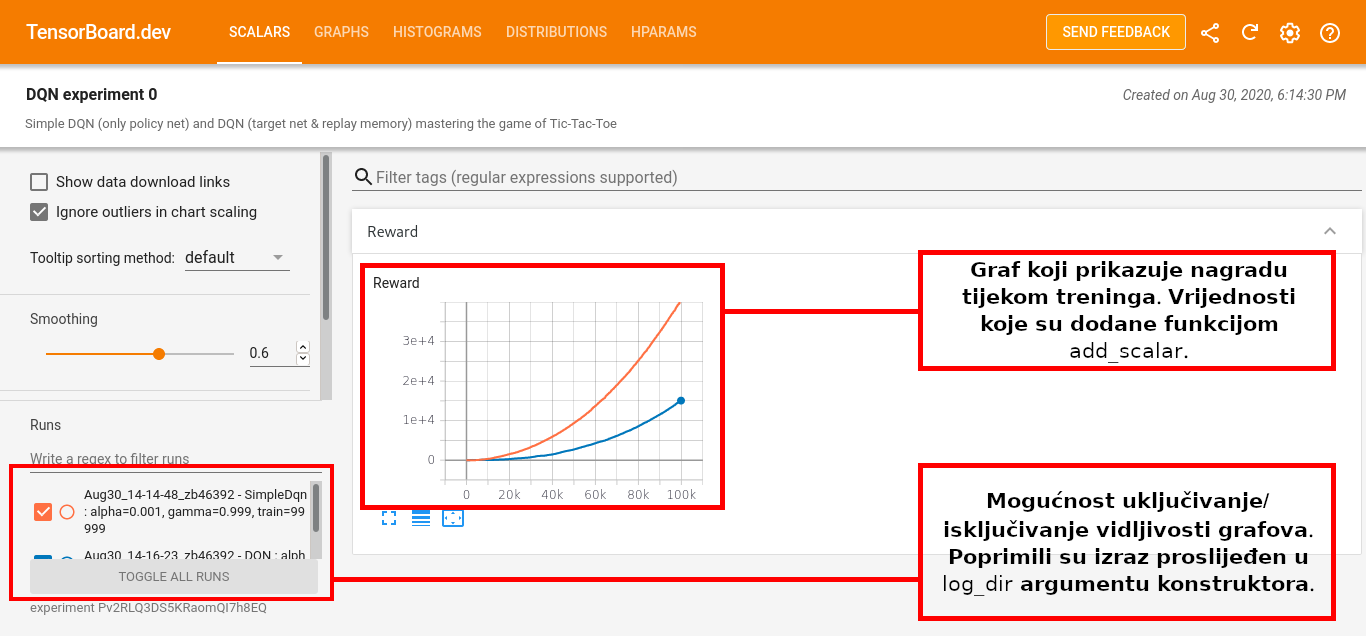
\includegraphics[width=0.8\linewidth,clip=]{images/tensorboard_00_edit.png}%
	\figcaption{Izgled Tensorboard vizualizacija mjernih podataka.}%
	\label{fig:tensorboard_00}%
\end{minipage}
\\[\intextsep]

Nakon poziva konstruktora poziva se funkcija \pythoninline{add_graph} koja zabilježava arhitekturu modela te podatke koje prima. Izgled tog područja prikazan je slikom~\ref{fig:tensorboard_01}. Dalje se tokom učenja agenta zabilježava zbroj svih nagrada u nekom trenutku sa funkcijom \pythoninline{add_scalar}, koji prima naziv vrijednosti, te sama vrijednost i korak u kojemu je postignuta ta vrijednost. Graf nagrade se nalazi na početnom području Tensorboarda vidljiv na slici~\ref{fig:tensorboard_00}. 
\\[\intextsep]
\begin{minipage}{\linewidth}
	\centering%
	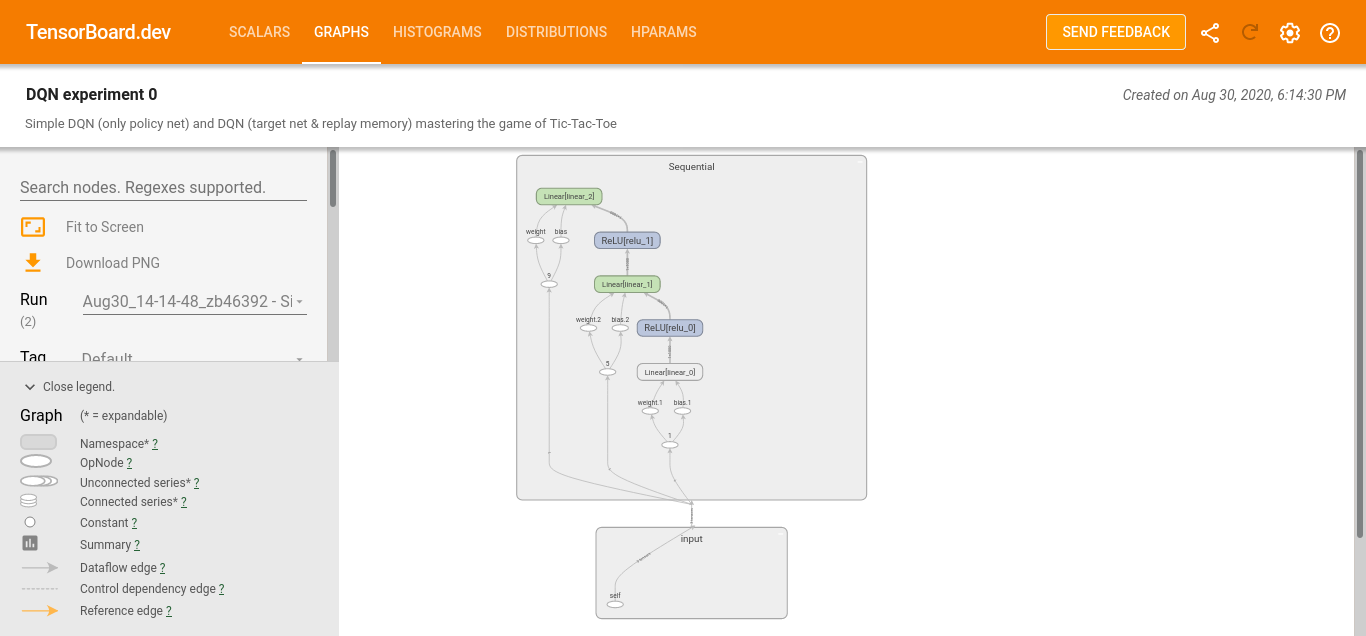
\includegraphics[width=0.8\linewidth,clip=]{images/tensorboard_01.png}%
	\figcaption{Tensorboard graf modela i njegovi slojevi.}%
	\label{fig:tensorboard_01}%
\end{minipage}
\\[\intextsep]

Dodatno se tokom učenja zabilježavaju i histogram parametra kako se mijenja, a to je moguće sa funkcijom \pythoninline{add_histogram}. Parametri koje ta funkcija prima su slični kako i kod \pythoninline{add_scalar}, samo što se ne radi o jednoj vrijednosti nego o skupu vrijednosti. Prikaz histograma i njihova distribucija u Tensorboardu su prikazani slikama~\ref{fig:tensorboard_02} i ~\ref{fig:tensorboard_03}.
\\[\intextsep]
\begin{minipage}{\linewidth}
	\centering%
	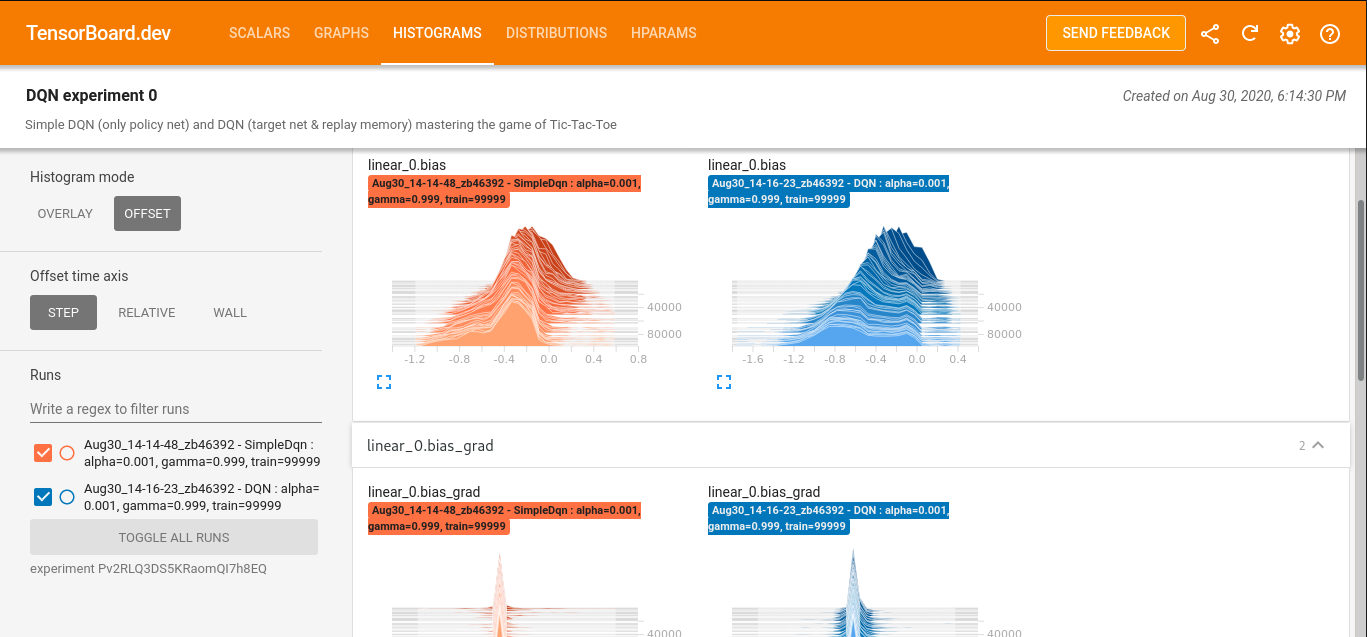
\includegraphics[width=0.8\linewidth,clip=]{images/tensorboard_02.png}%
	\figcaption{Tensorboard histogrami o vrijednostima u pojedinim slojevima.}%
	\label{fig:tensorboard_02}%
\end{minipage}
\\[\intextsep]
\begin{minipage}{\linewidth}
	\centering%
	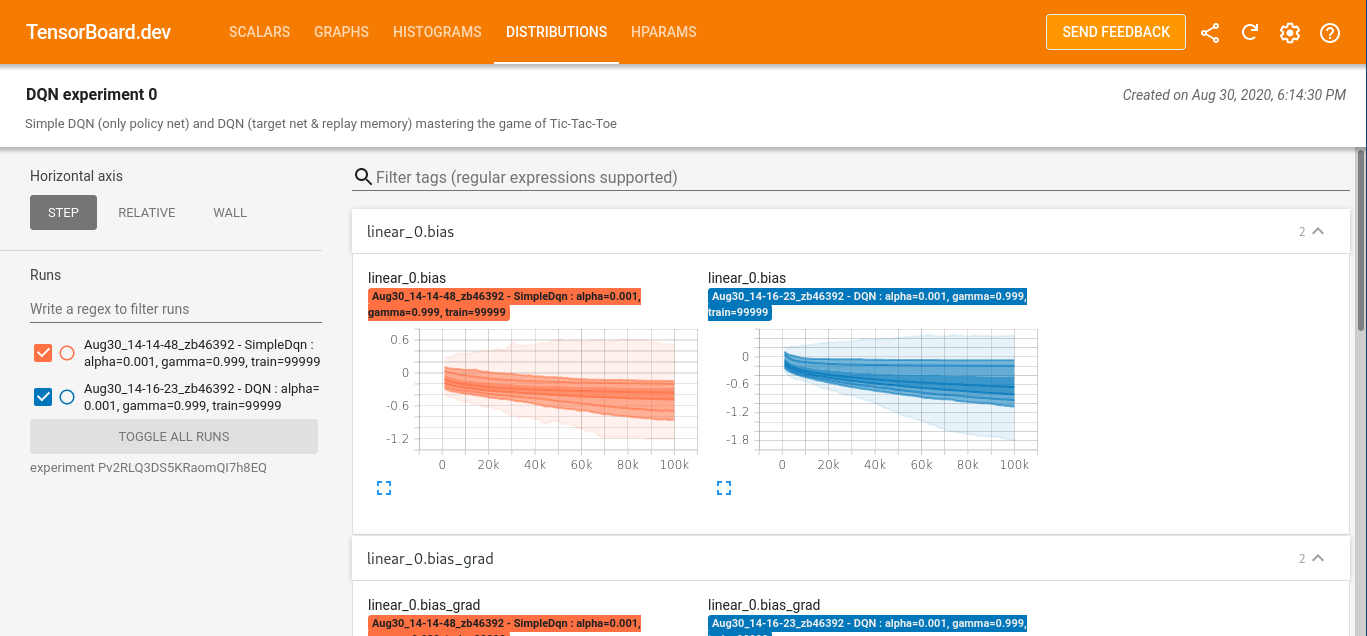
\includegraphics[width=0.8\linewidth,clip=]{images/tensorboard_03.png}%
	\figcaption{Tensorboard distribucije o vrijednostima u pojedinim slojevima.}%
	\label{fig:tensorboard_03}%
\end{minipage}
\\[\intextsep]

\subsection{Računalni oblak}
Učenje je dugotrajan proces, čak i sa suvremenim osobnim računalima. Tako da su se koristile dodatne računalne snage u oblaku, što može ubrzati proces učenja. Osim toga, što je veći broj računalne snage na raspolaganju mogu i više različitih algoritama istovremeno učiti. Postoje razni ponuđači koji nude mogućnost učenja u oblaku, međutim ovisno o snazi i prostoru pojedinog komponenta računala, se plaća određena cijena. Pronađene su mogućnosti korištenja računalnih oblaka koji se ne plaćaju, ali imaju druga ograničenja. Bez obzira na njih, u svrhu ovoga rada, bili su sasvim dovoljni za korištenje. Jedan od korištenih je Google Colaboratory, koji je izrađen od tvrtke Google. Radno sučelje jako liči na jupyter notebook. Jupyter notebook je alat za pisanje programskog k\^oda gdje se k\^od piše u ćelije. Svaka se ćelija može posebno pokrenuti, što omogućuje brze promjene bez da se cijeli k\^od iz početka pokreće. Dodatno se u ćelije mogu i pisati Markdown oznake uz pomoć kojih se izvršavane ćelije ispravno formatiraju. Ovo omogućuje da se programski k\^od i dokumentacija može nalaziti na istemu mjestu. Za korištenje Google Colaboratory alata, kako i za korištenje bilo kojeg Google alata, potrbno je izraditi Google korisnički račun. Izgled Google Colaboratory radnog sučelja prikazan je na slici~\ref{fig:google_colab}.
\\[\intextsep]
\begin{minipage}{\linewidth}
	\centering%
	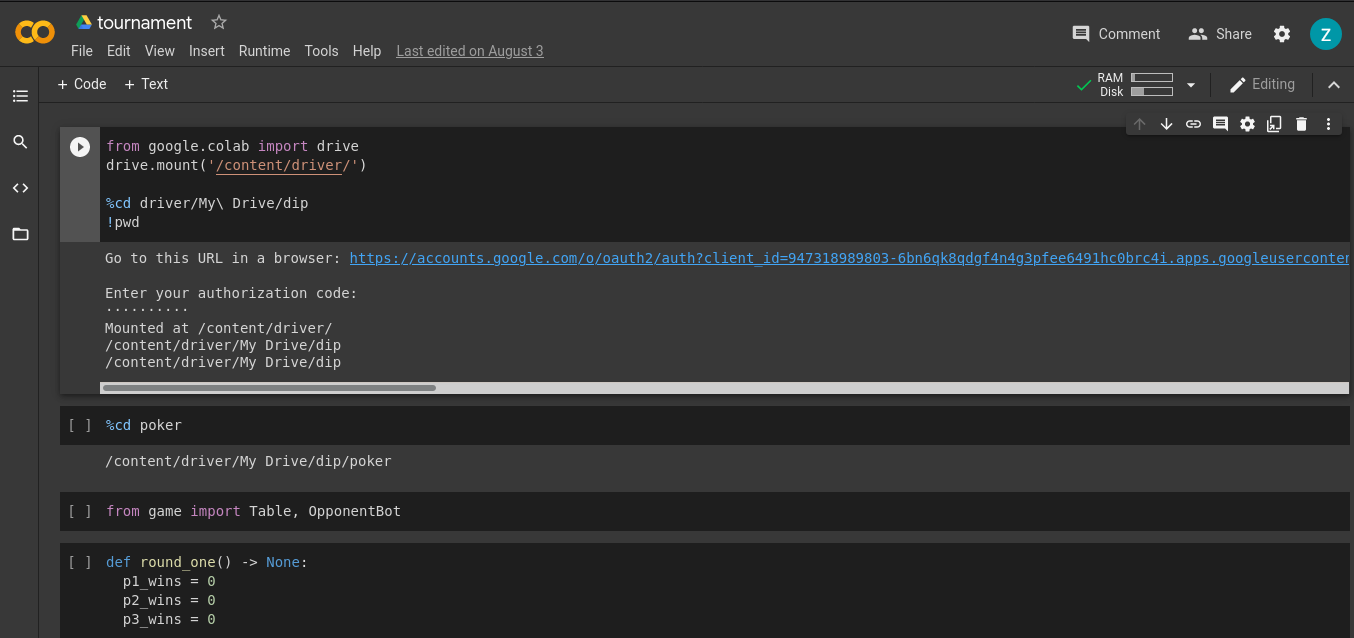
\includegraphics[width=0.8\linewidth,clip=]{images/google_colaboratory.png}%
	\figcaption{Radno okruženje Google Colaboratory.}%
	\label{fig:google_colab}%
\end{minipage}
\\[\intextsep]
Ograničenja u korištenju bez plaćanja, su mogućnost korištenja grafičke procesorske jedinice samo na jedan dan i Google Colaboratory mora u web pregledniku biti aktivan. Nakon nekog vremena neaktivnosti se svi procesi prekidaju. Zapravo omogućuju izvršenje puno kratkih procesa, a ne jednog koji se vrti jako dugo. Druga usluga računalnog oblaka koja je korištena je Paperspace. Ovdje se nudi korištenje grafičke procesorske jedinice 6 sati bez plaćanja. Nakon isteka tog vremena, oblak se ruši bez mogućnosti nastavka korištenja istog. Može se novoga pokrenuti, međutim nisu uvjek svi resursi slobodni, kako ih drugi korisnici rezerviraju. Prvo se izabere koji će radni okviri biti unaprijed instalirani i onda se izabere model grafičke kartice. Nakon sastavljanja željenog oblaka podiže se JupyterLab radno okruženje vidljivo na slici~\ref{fig:paperspace}.
\\[\intextsep]
\begin{minipage}{\linewidth}
	\centering%
	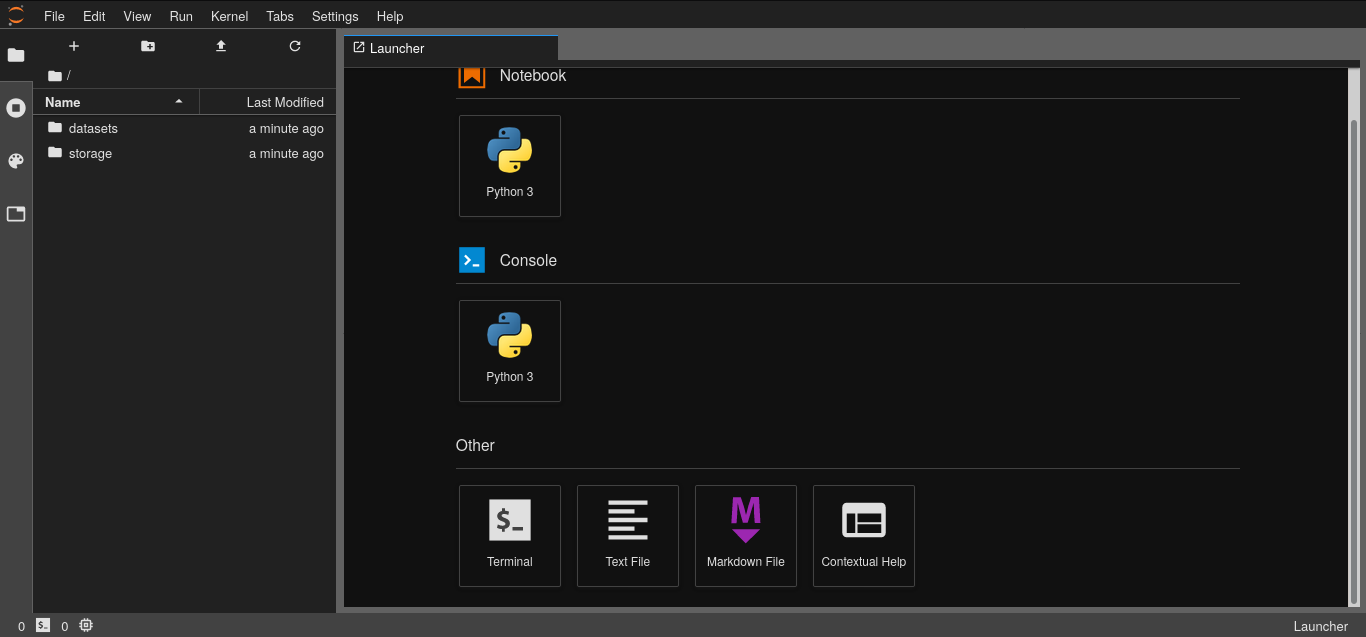
\includegraphics[width=0.8\linewidth,clip=]{images/paperspace.png}%
	\figcaption{Radno okruženje JupyterLab.}%
	\label{fig:paperspace}%
\end{minipage}
\\[\intextsep]
Može se primjetiti da u JupyterLab postoji mogućnost, osim otvarati Jupyter Notebook dokumente, otvoriti sučelje naredbenog redka (eng. \textit{command line interface}). Korištenje sučelja naredbenog redka je dosta pojednostavnilo korištenje oblaka u odnosu na jupyter notebook koji se u paperspace nije ni koristio. Moguće je u jupyter notebook izvršavati naredbe ljuske ako se na početak naredbe stavi uskličnik, npr. \pythoninline{\!pwd} koja ispisuje potpunu putanju do trenutačnog radnog direktorija. Za korištenje usluge kod Paperspace potrebno je izraditi korisnički račun, ili se može pak prijaviti sa korisničkom računom od Google ili GitHub.